\documentclass{article}
\usepackage[landscape,scale=.8]{geometry}

\usepackage{tikz}
\usetikzlibrary{braids}

\begin{document}
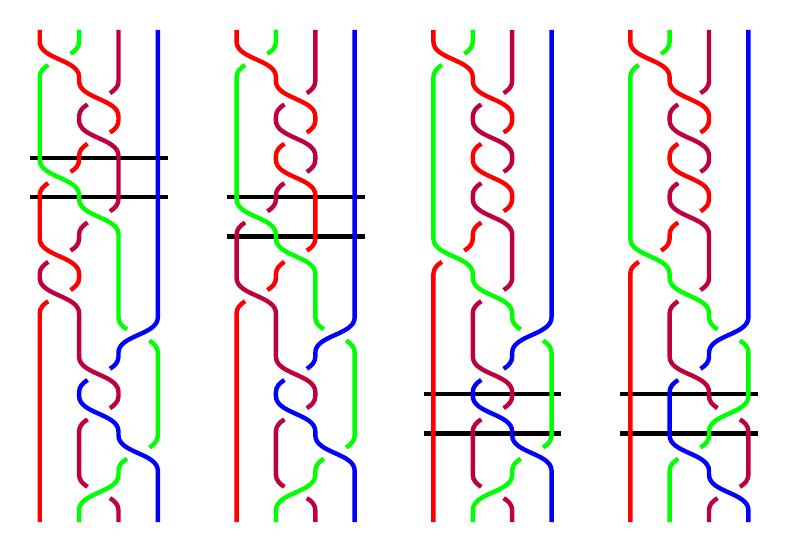
\begin{tikzpicture}[
  scale=.5,
  ultra thick,
  braid/strand 1/.style={red},
  braid/strand 2/.style={green},
  braid/strand 3/.style={purple},
  braid/strand 4/.style={blue},
  braid/every floor/.style={draw},
  braid/gap=.2,
]
\pic[name prefix=braid,transform shape]
{braid={s_1 s_2 s_2 |-{3} s_1 s_2 s_1 s_1 s_3^{-1} s_2 s_2 s_3 s_2^{-1}}};
\pic[name prefix=braid,transform shape] at (5,0)
{braid={s_1 s_2 s_2 s_2 |-{3} s_1 s_2 s_1 s_3^{-1} s_2 s_2 s_3 s_2^{-1}}};
\pic[name prefix=braid,transform shape] at (10,0)
{braid={s_1 s_2 s_2 s_2 s_2 s_1 s_2 s_3^{-1} s_2 |-{3} s_2 s_3 s_2^{-1}}};
\pic[name prefix=braid,transform shape] at (15,0)
{braid={s_1 s_2 s_2 s_2 s_2 s_1 s_2 s_3^{-1} s_2 |-{2} s_3^{-1} s_2 s_3}};
\end{tikzpicture}

\end{document}
